\documentclass[conference]{IEEEtran}
\usepackage{amsmath,amssymb,amsfonts}
\usepackage{graphicx}
% Resolves figures/ whether compiled from the repo root or from paper/
\graphicspath{{./}{../}}
\usepackage{textcomp}
\usepackage{booktabs}
\usepackage{cite}
\usepackage{hyperref}

\begin{document}

\title{Beyond Point Estimates: Bayesian Gaussian Process Inference for In-Game Win Probability with Uncertainty Quantification}

\author{
\IEEEauthorblockN{Lord Joshua E. Lacuata}
\IEEEauthorblockA{College of Engineering \\
University of the Philippines Diliman \\
Quezon City, Philippines \\
lordjoshualacuata@gmail.com}
}

\maketitle

\begin{abstract}
In-game win probability models have become standard analytical tools in professional basketball, yet all widely deployed implementations produce point estimates that suppress information about predictive confidence. This study applies Bayesian inference via Gaussian Process (GP) regression to estimate the full posterior predictive distribution of win probability conditioned on in-game state, yielding both a probability estimate and a calibrated credible interval at every moment of a game. Using 174,050 game-state observations sampled from 6,962 NBA regular season games across the 2018--19 through 2023--24 seasons, we compare the GP against three frequentist baselines: simple logistic regression, polynomial logistic regression, and XGBoost. Bayesian model selection via log marginal likelihood identifies a composite RBF + Mat\'{e}rn 1.5 kernel as the optimal prior, with optimized mixing weights revealing that win probability is approximately 93\% smooth with 7\% roughness. On the held-out 2023--24 season, the GP achieves a log-loss of 0.4831 and Brier score of 0.1636, within 0.007 log-loss of XGBoost, while providing 95\% credible intervals that achieve 80\% empirical coverage. An uncertainty decomposition across game contexts reveals that blowout states carry high epistemic uncertainty but low aleatoric uncertainty, while clutch states exhibit the inverse pattern, a structural distinction invisible to point-estimate models.
\end{abstract}

\begin{IEEEkeywords}
Gaussian Process, Bayesian Inference, Uncertainty Quantification, Win Probability, NBA, Sports Analytics.
\end{IEEEkeywords}

% ============================================================
\section{Introduction}
% ============================================================

The estimation of in-game win probability has evolved from a niche statistical exercise into a central component of modern sports analytics infrastructure. Major broadcasting networks overlay real-time win probability curves during live game coverage, front offices use probability-based frameworks to evaluate coaching decisions post hoc, and sports betting markets increasingly rely on live models to set in-game lines. In the NBA specifically, platforms such as ESPN, NBA.com, and FiveThirtyEight have deployed win probability trackers that update after every play, providing viewers and analysts with a dynamic measure of which team is more likely to prevail.

Despite widespread adoption, a fundamental limitation persists across all major implementations: they output a single point estimate at each game state. When the model reports a 73\% home win probability with 4 minutes remaining, it communicates nothing about how confident that estimate is. A 73\% prediction derived from a game state observed thousands of times carries fundamentally different informational content than a 73\% prediction extrapolated to a rarely seen scenario, yet point-estimate models treat both identically.

This limitation has practical consequences. Coaching staffs making strategic decisions based on win probability, such as whether to call a timeout or engage in tactical fouling, would benefit from knowing whether the model's recommendation is grounded in dense historical precedent or is an uncertain extrapolation. Similarly, in-game betting markets would benefit from probability estimates accompanied by confidence bands that reflect the model's epistemic state.

The Bayesian statistical framework offers a natural resolution. Rather than estimating a single function that maps game state to win probability, Bayesian inference maintains a posterior distribution over the space of possible functions. Predictions emerge as integrals over this posterior, yielding both a mean estimate and a variance that quantifies the model's uncertainty. Gaussian Processes \cite{rasmussen2006} instantiate this framework with particular elegance: the prior over functions is specified through a kernel function, the posterior is obtained in closed form, and predictions at new inputs come equipped with analytically derived credible intervals.

This study applies GP regression to NBA in-game win probability estimation, operating on a compact two-dimensional input space of score margin and time remaining. The contribution is threefold: (1) we demonstrate that a GP achieves predictive accuracy within 0.007 log-loss of XGBoost while additionally providing calibrated posterior uncertainty; (2) we show through Bayesian model selection that a composite RBF + Mat\'{e}rn 1.5 kernel optimally represents win probability dynamics, with interpretable mixing weights; and (3) we introduce an epistemic-aleatoric uncertainty decomposition that reveals structurally different uncertainty profiles across game contexts.

% ============================================================
\section{Related Work}
% ============================================================

\subsection{Win Probability Modeling in Sports}

Quantitative win probability estimation has roots in Stern's Brownian motion model for baseball \cite{stern1994}, which treated the evolution of run differential as a stochastic process and derived win probability as a function of current state and remaining time. Lock and Nettleton \cite{lock2014} generalized this framework to multiple sports, demonstrating that logistic regression models conditioned on score differential and game clock provide well-calibrated estimates across NFL, NBA, and NHL data. Their work established the two-variable input space (margin, time remaining) as sufficient for competitive win probability modeling, a design decision adopted in this study.

In the NBA context, Cervone et al. \cite{cervone2016} introduced Expected Possession Value (EPV), a framework that models the probability of scoring outcomes at each moment using optical tracking data. Feature-analysis approaches to NBA outcome prediction, such as Thabtah et al. \cite{thabtah2019}, have shown that a small number of box-score-derived variables carries most of the predictive signal, reinforcing the case for compact input spaces. More recent implementations, including ESPN's proprietary model, rely on gradient-boosted decision trees, though their architectures remain undisclosed.

\subsection{Uncertainty Quantification in Predictive Modeling}

The distinction between epistemic uncertainty (reducible, arising from limited data) and aleatoric uncertainty (irreducible, inherent in the data-generating process) was formalized in the machine learning context by Kendall and Gal \cite{kendall2017}. Their framework demonstrates that conflating the two types produces misleading confidence estimates.

Gaussian Processes have been widely used for uncertainty-aware prediction in geostatistics, Bayesian optimization \cite{frazier2018}, and engineering design. Their application to sports analytics remains sparse. To our knowledge, no published work applies GP inference to in-game win probability estimation with explicit uncertainty quantification, representing the gap this study addresses.

% ============================================================
\section{Methodology}
% ============================================================

\subsection{Data Collection and Preprocessing}

Play-by-play event data was collected for all NBA regular season games from the 2018--19 through 2023--24 seasons via the \texttt{nba\_api} Python package, using the PlayByPlayV3 endpoint, as the V2 endpoint was deprecated during the data collection phase. Games played during the 2019--20 Orlando bubble (post-July 2020) were excluded due to the absence of home court advantage. The final dataset comprises 6,962 games.

For each game, the in-game state was sampled at 2-minute intervals throughout regulation (48 minutes), producing 24 observations per game at time points $t \in \{2880, 2760, \ldots, 120, 0\}$ seconds remaining. At each sample point, the most recent score was extracted and the margin computed as $m = s_{\text{home}} - s_{\text{away}}$. Overtime periods were excluded. Each observation was paired with a binary label $y \in \{0, 1\}$ indicating whether the home team won.

The resulting dataset contains 174,050 game-state observations. A strict temporal split was applied: seasons 2018--19 through 2022--23 (5,732 games, 143,300 observations) for training, and 2023--24 (1,230 games, 30,750 observations) for testing. Zero game overlap exists between splits.

For GP training, the observation-level data was aggregated into a two-dimensional grid. Score margin was binned in 2-point increments from $-30$ to $+30$, and time remaining in 120-second increments. Within each bin, the empirical home win rate $\hat{p}$ and observation count $n$ were computed. Bins with fewer than 5 observations were discarded, yielding 634 training points with a mean of 226 observations per bin.

\subsection{Bayesian Inference via Gaussian Processes}

A Gaussian Process defines a probability distribution over functions $f: \mathcal{X} \to \mathbb{R}$, specified by a mean function $\mu(\mathbf{x})$ and a covariance function $k(\mathbf{x}, \mathbf{x}')$ \cite{rasmussen2006, pilario2023}:
%
\begin{equation}
f(\mathbf{x}) \sim \mathcal{GP}\big(\mu(\mathbf{x}),\, k(\mathbf{x}, \mathbf{x}')\big)
\end{equation}

For a training set $\{\mathbf{X}, \mathbf{y}\}$ with observations corrupted by additive Gaussian noise $\epsilon \sim \mathcal{N}(0, \sigma_n^2)$, the posterior predictive distribution at a new input $\mathbf{x}_*$ is Gaussian with mean and variance:
%
\begin{equation}
\mu_* = \mathbf{k}_*^T (\mathbf{K} + \sigma_n^2 \mathbf{I})^{-1} \mathbf{y}
\label{eq:gp_mean}
\end{equation}
%
\begin{equation}
\sigma_*^2 = k(\mathbf{x}_*, \mathbf{x}_*) - \mathbf{k}_*^T (\mathbf{K} + \sigma_n^2 \mathbf{I})^{-1} \mathbf{k}_*
\label{eq:gp_var}
\end{equation}
%
where $\mathbf{K}$ is the $n \times n$ kernel matrix with $K_{ij} = k(\mathbf{x}_i, \mathbf{x}_j)$, and $\mathbf{k}_* = [k(\mathbf{x}_*, \mathbf{x}_1), \ldots, k(\mathbf{x}_*, \mathbf{x}_n)]^T$. The posterior mean $\mu_*$ provides the point prediction, while $\sigma_*^2$ quantifies the model's uncertainty at $\mathbf{x}_*$.

In this study, inputs are $\mathbf{x} = (m, t)$ where $m$ is binned score margin and $t$ is binned time remaining. The target is the empirical win rate $\hat{p} \in [0, 1]$. We employ GP regression on continuous win rates rather than GP classification on binary outcomes, as the binning procedure transforms the problem into regression with observation noise \cite{bishop2006}.

\subsection{Kernel Selection via Marginal Likelihood}

The kernel function encodes prior beliefs about the structure of the win probability surface. Five candidate kernels were evaluated:

\begin{equation}
k_{\text{RBF}}(\mathbf{x}, \mathbf{x}') = \sigma_f^2 \exp\!\left(-\frac{\|\mathbf{x} - \mathbf{x}'\|^2}{2\ell^2}\right)
\end{equation}

\begin{equation}
k_{\text{Mat}}(\mathbf{x}, \mathbf{x}') = \sigma_f^2 \frac{2^{1-\nu}}{\Gamma(\nu)} \left(\frac{\sqrt{2\nu}\,r}{\ell}\right)^\nu K_\nu\!\left(\frac{\sqrt{2\nu}\,r}{\ell}\right)
\end{equation}

\begin{equation}
k_{\text{RQ}}(\mathbf{x}, \mathbf{x}') = \sigma_f^2 \left(1 + \frac{\|\mathbf{x} - \mathbf{x}'\|^2}{2\alpha \ell^2}\right)^{-\alpha}
\end{equation}
%
where $r = \|\mathbf{x} - \mathbf{x}'\|$, $\ell$ is the length scale, $\sigma_f^2$ the signal variance, $\nu$ controls roughness, and $K_\nu$ is the modified Bessel function.

The five candidates are: (i) RBF, (ii) Mat\'{e}rn $\nu\!=\!2.5$, (iii) Mat\'{e}rn $\nu\!=\!1.5$, (iv) Rational Quadratic, and (v) a composite $k_5 = c_1 \cdot k_{\text{RBF}} + c_2 \cdot k_{\text{Mat\,1.5}}$. Model selection proceeds via the log marginal likelihood (LML):
%
\begin{equation}
\log p(\mathbf{y} | \mathbf{X}, \boldsymbol{\theta}) = -\frac{1}{2}\mathbf{y}^T\mathbf{K}_\theta^{-1}\mathbf{y} - \frac{1}{2}\log|\mathbf{K}_\theta| - \frac{n}{2}\log 2\pi
\label{eq:lml}
\end{equation}
%
The LML balances data fit against model complexity, implementing an automatic Occam's razor \cite{rasmussen2006}. Hyperparameters are optimized via L-BFGS-B with 10 random restarts.

\subsection{Noise Calibration}

Binned win rates carry unmodeled variance from factors absent in the two-dimensional input space: team quality differentials, injury status, rest days, and referee assignments. To prevent overconfidence, a bounded WhiteKernel with noise level constrained to $[0.01, 1.0]$ was employed alongside diagonal regularization $\alpha = 0.01$. This forces the GP to maintain a minimum noise floor, ensuring the posterior variance remains informative.

Because the GP is fitted in an unconstrained real-valued output space, the posterior mean and the endpoints of every credible interval were clipped to the $[0, 1]$ range to respect the probability domain.

\subsection{Baseline Models}

Three frequentist baselines were trained on the same features $(m, t)$ using unbinned training data:

\textbf{Simple Logistic Regression.} Standard logistic regression with $\ell_2$ regularization, modeling $P(y\!=\!1 | m, t) = \sigma(\mathbf{w}^T\mathbf{x} + b)$ \cite{pilario2023}.

\textbf{Polynomial Logistic Regression.} Degree-3 polynomial expansion including the interaction term $mt$, capturing the dependence of margin significance on time remaining \cite{pilario2023}.

\textbf{XGBoost.} Gradient-boosted decision trees (200 estimators, max depth 4, learning rate 0.1), serving as a strong nonparametric baseline \cite{chen2016}.

All features were standardized to zero mean and unit variance prior to training. Preprocessing, the logistic regression baselines, the polynomial basis expansion, the Gaussian Process implementation, and all evaluation metrics use \texttt{scikit-learn} \cite{pedregosa2011}.

% ============================================================
\section{Results}
% ============================================================

\subsection{Exploratory Data Analysis}

The training dataset exhibits the expected structural properties of NBA game-state data. The score margin distribution is approximately Gaussian, centered near zero with a slight rightward skew reflecting home court advantage (overall home win rate: 56.0\%). The empirical win rate as a function of score margin follows a sigmoid curve, crossing 50\% near margin zero and approaching saturation beyond $\pm 20$ points.

% === FIGURE: EDA Plots ===
\begin{figure*}[!t]
\centering
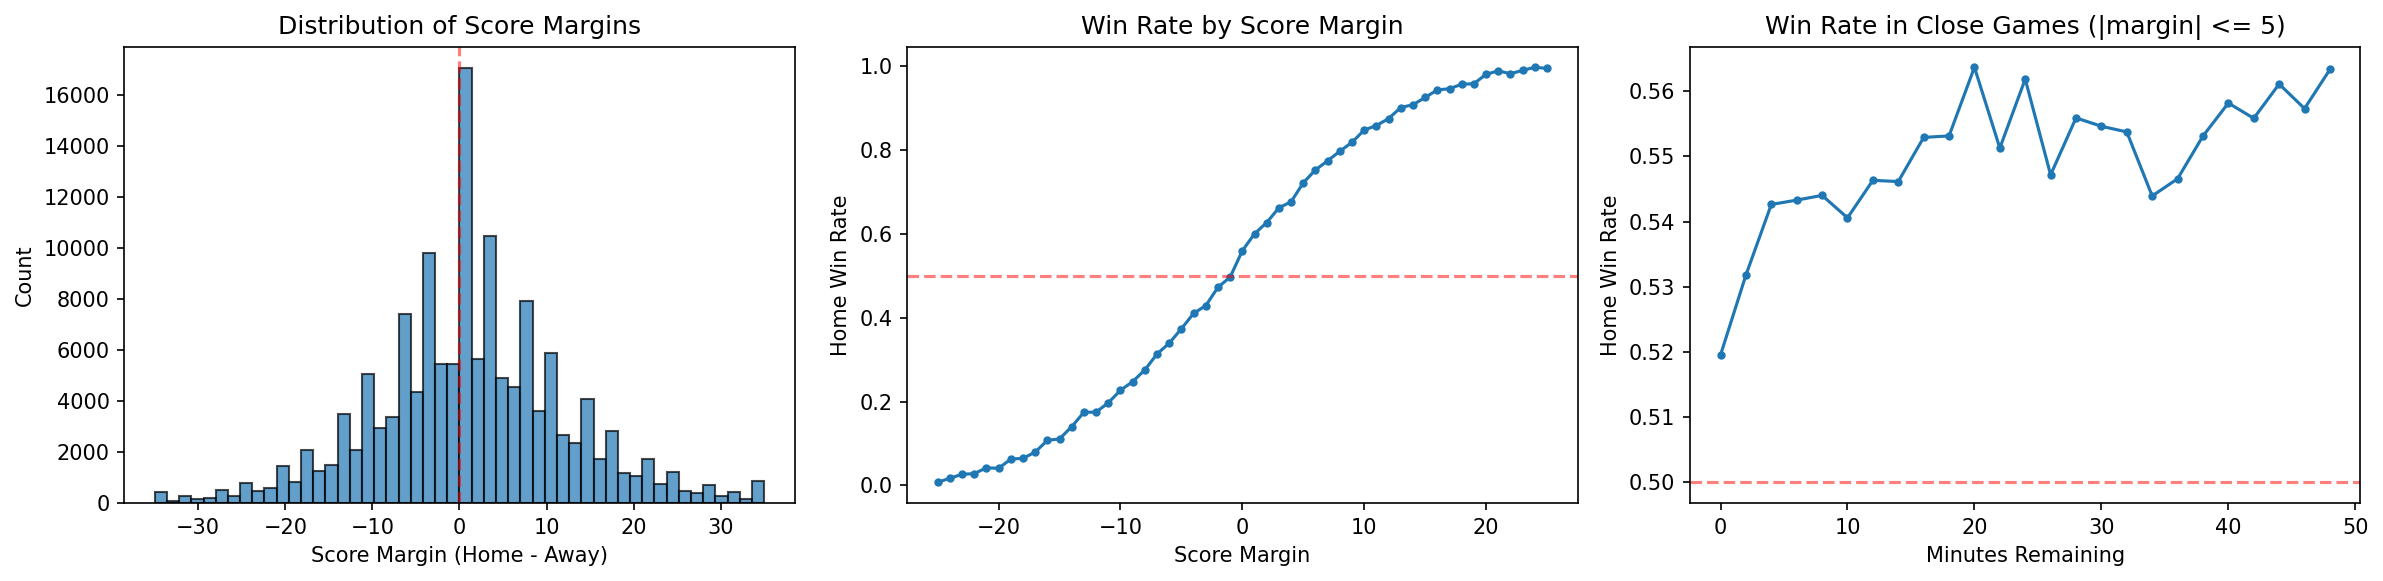
\includegraphics[width=0.92\textwidth]{figures/01_eda_checks.png}
\caption{Exploratory data analysis of the training set. Left: score margin distribution. Center: win rate by score margin (sigmoid curve). Right: win rate in close games ($|m| \leq 5$) by minutes remaining.}
\label{fig:eda}
\end{figure*}

The empirical win rate heatmap across the full $(m, t)$ grid confirms monotonic behavior: high win probability at positive margins intensifying as time decreases, with symmetric behavior at negative margins. White cells at extreme margins in early-game regions reflect data sparsity.

% === FIGURE: Empirical Heatmap ===
\begin{figure}[!t]
\centering
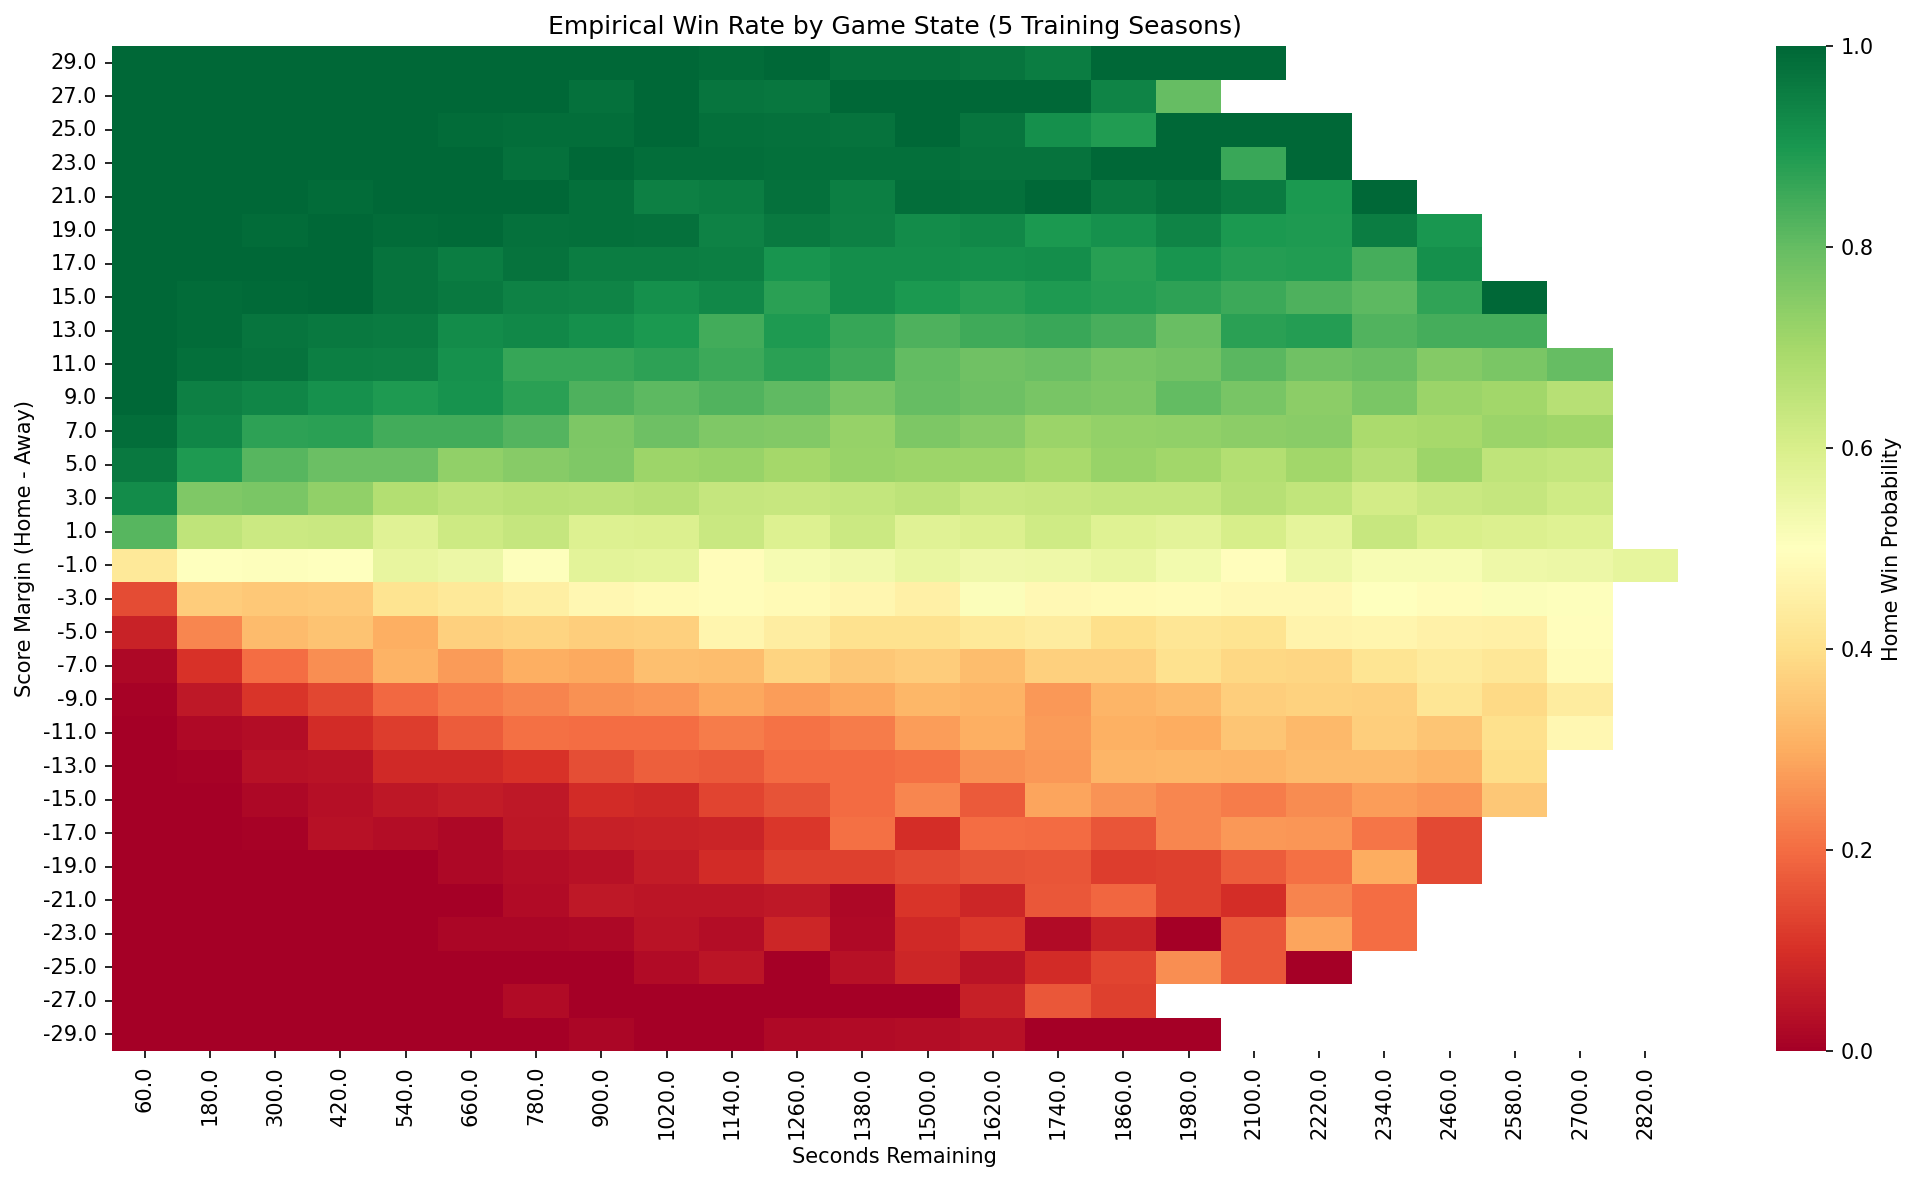
\includegraphics[width=\columnwidth]{figures/01_empirical_heatmap.png}
\caption{Empirical win rate by game state across five training seasons (2018--19 through 2022--23). Green indicates high home win probability, red indicates low.}
\label{fig:heatmap}
\end{figure}

\subsection{Bayesian Model Selection}

Table~\ref{tab:kernels} presents the log marginal likelihood comparison across five candidate kernels. The composite RBF + Mat\'{e}rn 1.5 kernel achieves the highest LML, indicating that win probability is best represented as a mixture of smooth and moderately rough components.

\begin{table}[t]
\centering
\caption{Kernel Comparison via Log Marginal Likelihood}
\label{tab:kernels}
\begin{tabular}{lc}
\toprule
\textbf{Kernel} & \textbf{Log Marginal Likelihood} \\
\midrule
RBF + Mat\'{e}rn 1.5 & \textbf{589.68} \\
Mat\'{e}rn 1.5 & 587.23 \\
Mat\'{e}rn 2.5 & 587.15 \\
RBF & 577.90 \\
Rational Quadratic & 557.74 \\
\bottomrule
\end{tabular}
\end{table}

The kernel structure was identified during this selection step and subsequently refitted with the calibrated noise model of Section~III-D for the final deployment. The optimized composite kernel takes the form:
%
\begin{equation}
\begin{split}
k_{\text{final}} = \underbrace{0.988^2 \cdot k_{\text{RBF}}(\ell\!=\![0.72, 4.99])}_{\text{93\% weight}} \\
+ \underbrace{0.262^2 \cdot k_{\text{Mat\,1.5}}(\ell\!=\![1.13, 2.94])}_{\text{7\% weight}} \\
+ k_{\text{White}}(\sigma_n^2\!=\!0.01)
\end{split}
\end{equation}

The percentages represent relative variance contributions after normalizing the squared mixing weights, which sum to 1.045 in their raw form.

The RBF component dominates ($0.988^2 = 0.976$), while Mat\'{e}rn 1.5 contributes $0.262^2 = 0.069$. Win probability is approximately 93\% smooth with 7\% roughness, the latter capturing sharper transitions near critical game states. The RBF length scales $[0.72, 4.99]$ indicate that score margin changes are significant over a shorter range than time remaining changes: a few-point scoring run alters win probability more sharply than an equivalent interval of game clock.

\subsection{Predictive Performance}

Table~\ref{tab:models} compares all four models on the held-out 2023--24 season.

\begin{table}[t]
\centering
\caption{Model Comparison on 2023--24 Test Season}
\label{tab:models}
\begin{tabular}{lccc}
\toprule
\textbf{Model} & \textbf{Log-Loss} & \textbf{Brier} & \textbf{Acc.} \\
\midrule
LR (simple) & 0.4998 & 0.1674 & 74.81\% \\
LR (poly deg 3) & 0.4804 & 0.1627 & 74.94\% \\
XGBoost & \textbf{0.4766} & \textbf{0.1618} & \textbf{74.97\%} \\
GP (RBF + Mat\'{e}rn 1.5) & 0.4831 & 0.1636 & 74.79\% \\
\bottomrule
\end{tabular}
\end{table}

XGBoost achieves the lowest log-loss and Brier score, outperforming the GP by 0.0065 and 0.0018 respectively. The GP performs comparably to polynomial logistic regression (log-loss difference of 0.0027). All models achieve similar accuracy in the 74.8--75.0\% range, reflecting a shared ceiling imposed by the two-feature input space. The GP's slight deficit relative to XGBoost is expected: tree-based models capture sharp nonlinear thresholds, while the GP enforces smoothness through its kernel prior. This tradeoff is central to the study's argument: the GP sacrifices marginal predictive performance in exchange for principled uncertainty quantification.

\subsection{GP Posterior Surfaces}

The GP posterior mean surface displays the expected structure: smooth probability gradients with contours tightening as time remaining decreases. The posterior standard deviation surface reveals higher uncertainty at extreme margins in early-game regions (sparse training data) and lower uncertainty in the dense central region.

% === FIGURE: GP Surfaces ===
\begin{figure*}[!t]
\centering
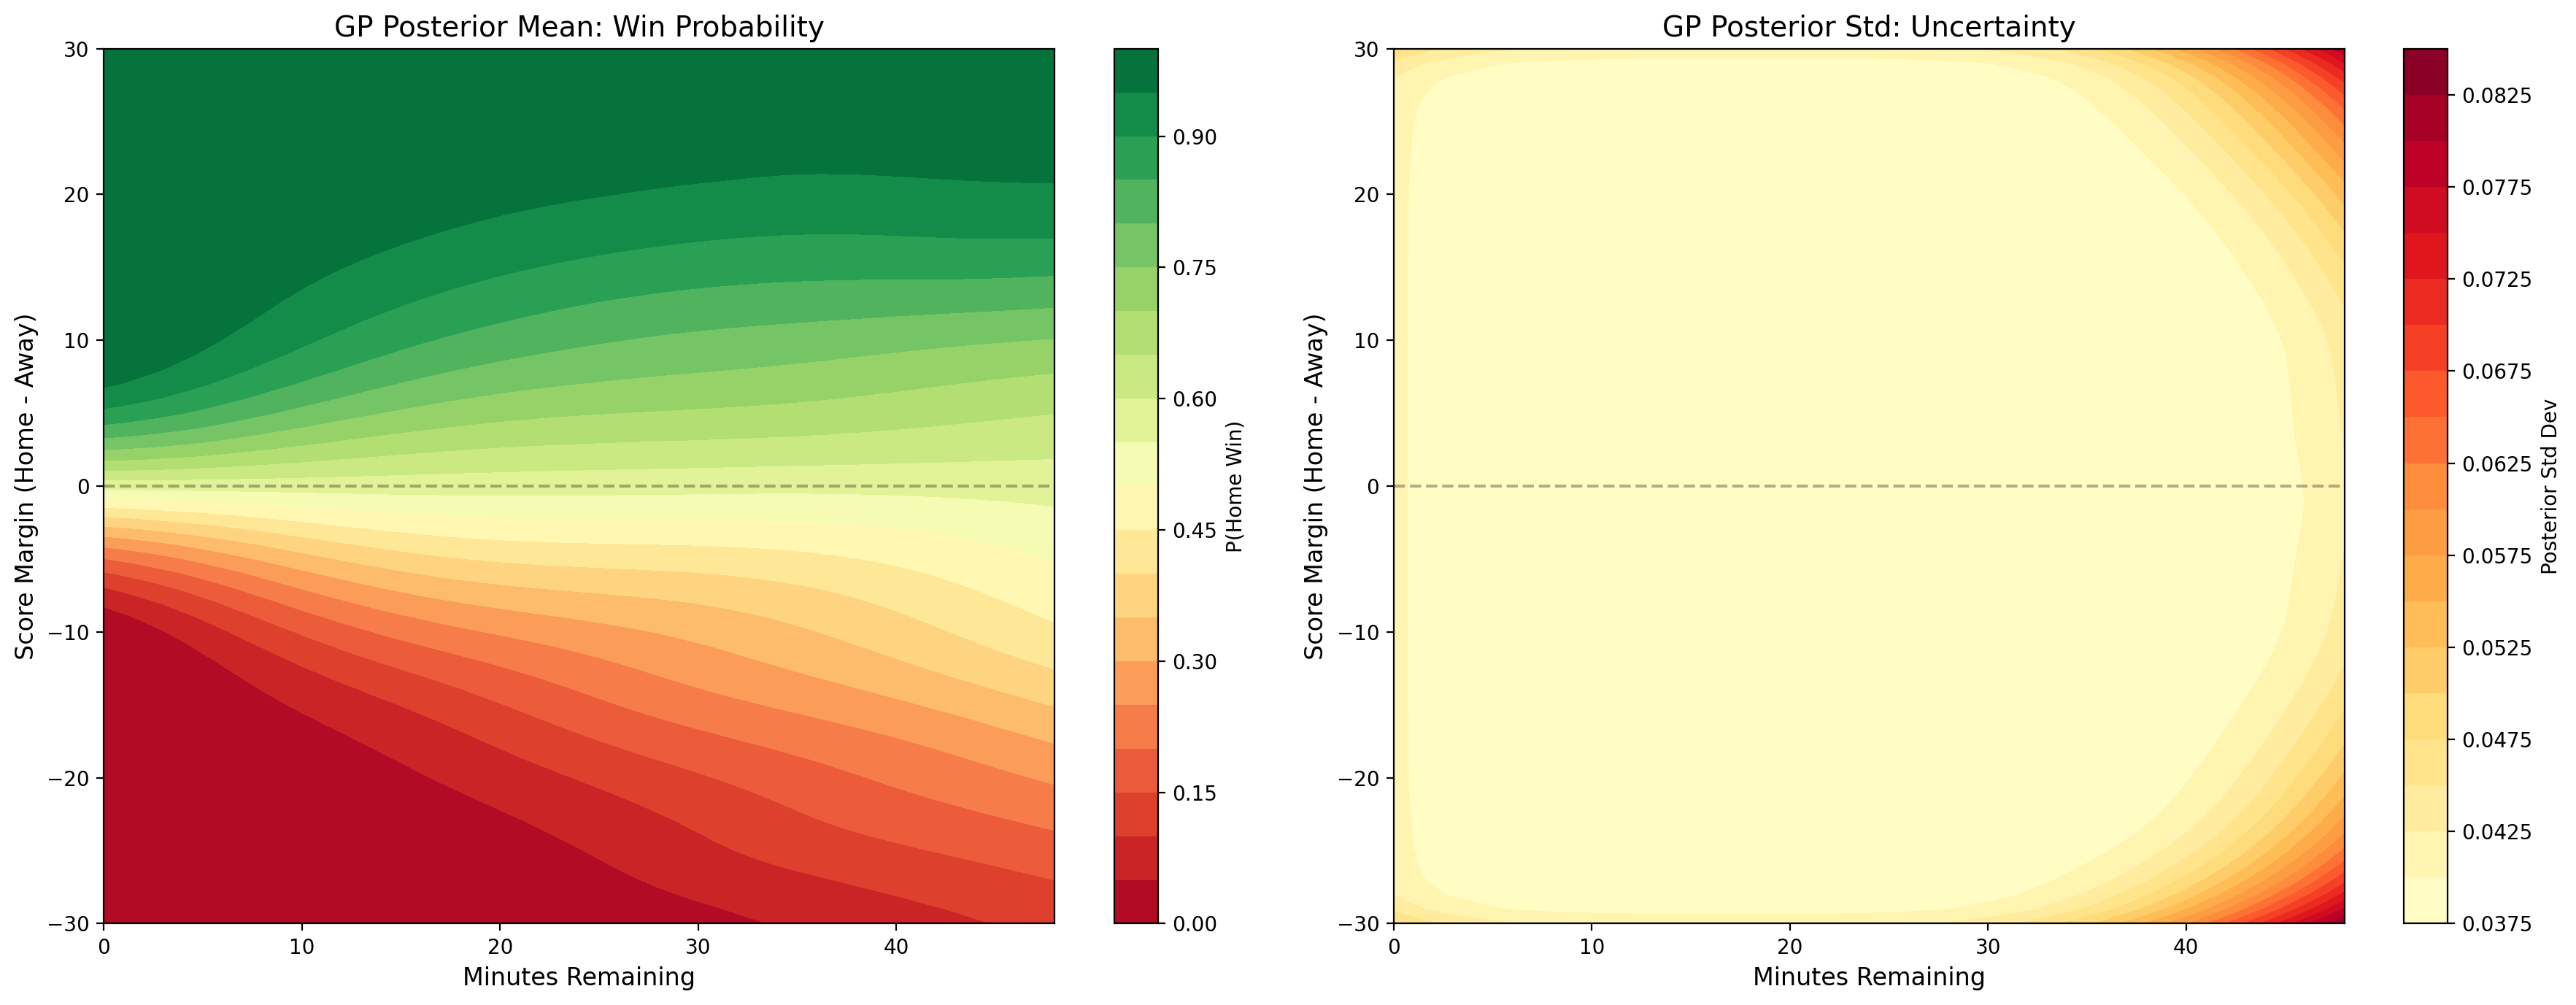
\includegraphics[width=0.92\textwidth]{figures/02_gp_surfaces.png}
\caption{GP posterior predictive surfaces. Left: posterior mean $\mu_*$ representing win probability. Right: posterior standard deviation $\sigma_*$ representing epistemic uncertainty.}
\label{fig:surfaces}
\end{figure*}

\subsection{Calibration Analysis}

The calibration curves for all four models track the diagonal closely, indicating well-calibrated probability estimates. The GP and polynomial logistic regression exhibit near-identical calibration behavior. Phase-specific analysis reveals that all models maintain calibration quality across first half, second half, and clutch time ($< 5$ minutes remaining).

% === FIGURE: Calibration Curves ===
\begin{figure}[!t]
\centering
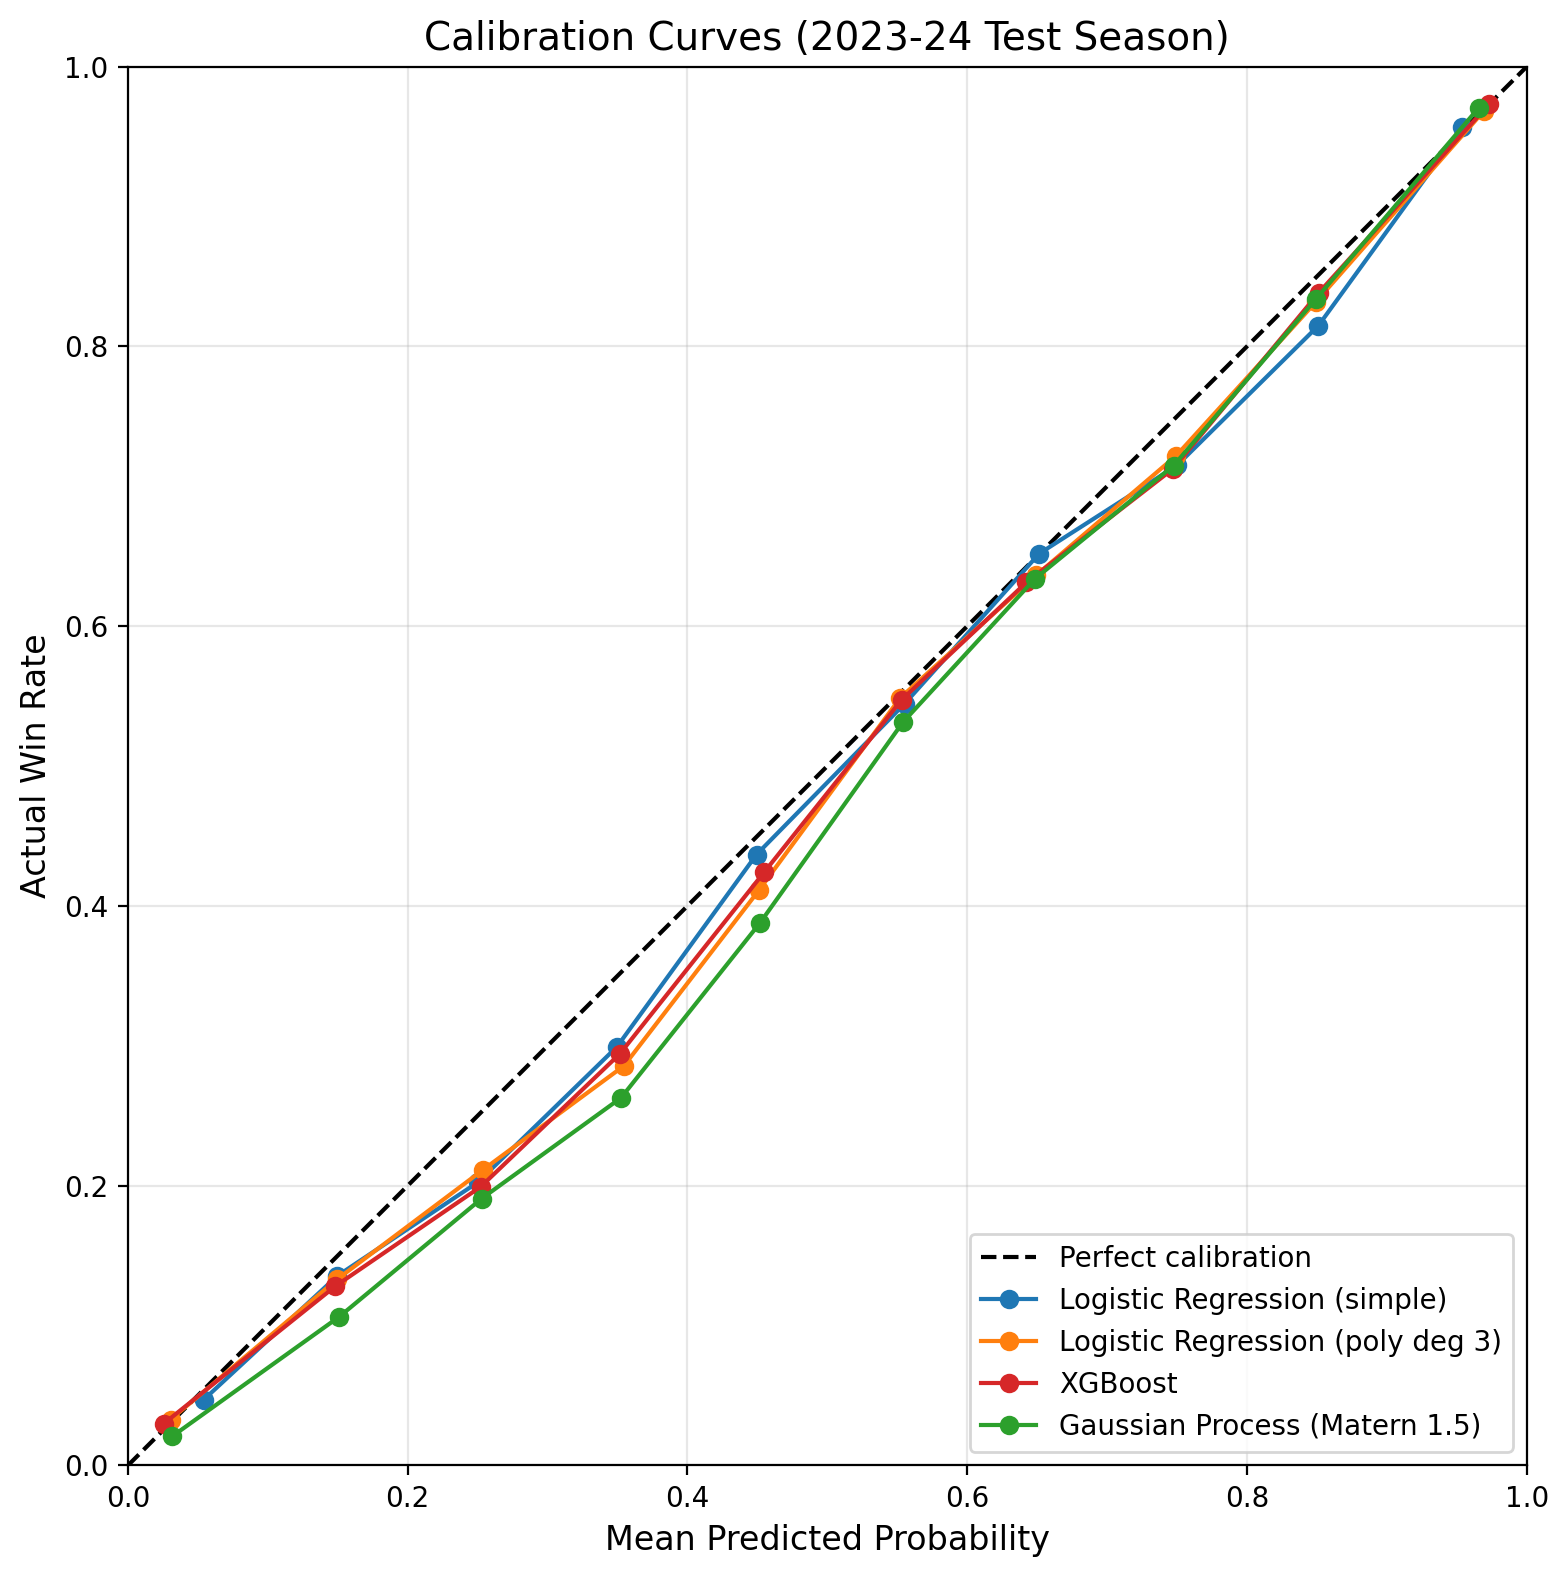
\includegraphics[width=\columnwidth]{figures/03_calibration_curves.png}
\caption{Calibration curves on the 2023--24 test season. All models track the diagonal, with the GP and polynomial LR showing near-identical behavior.}
\label{fig:calibration}
\end{figure}

% === FIGURE: Calibration by Phase ===
\begin{figure*}[!t]
\centering
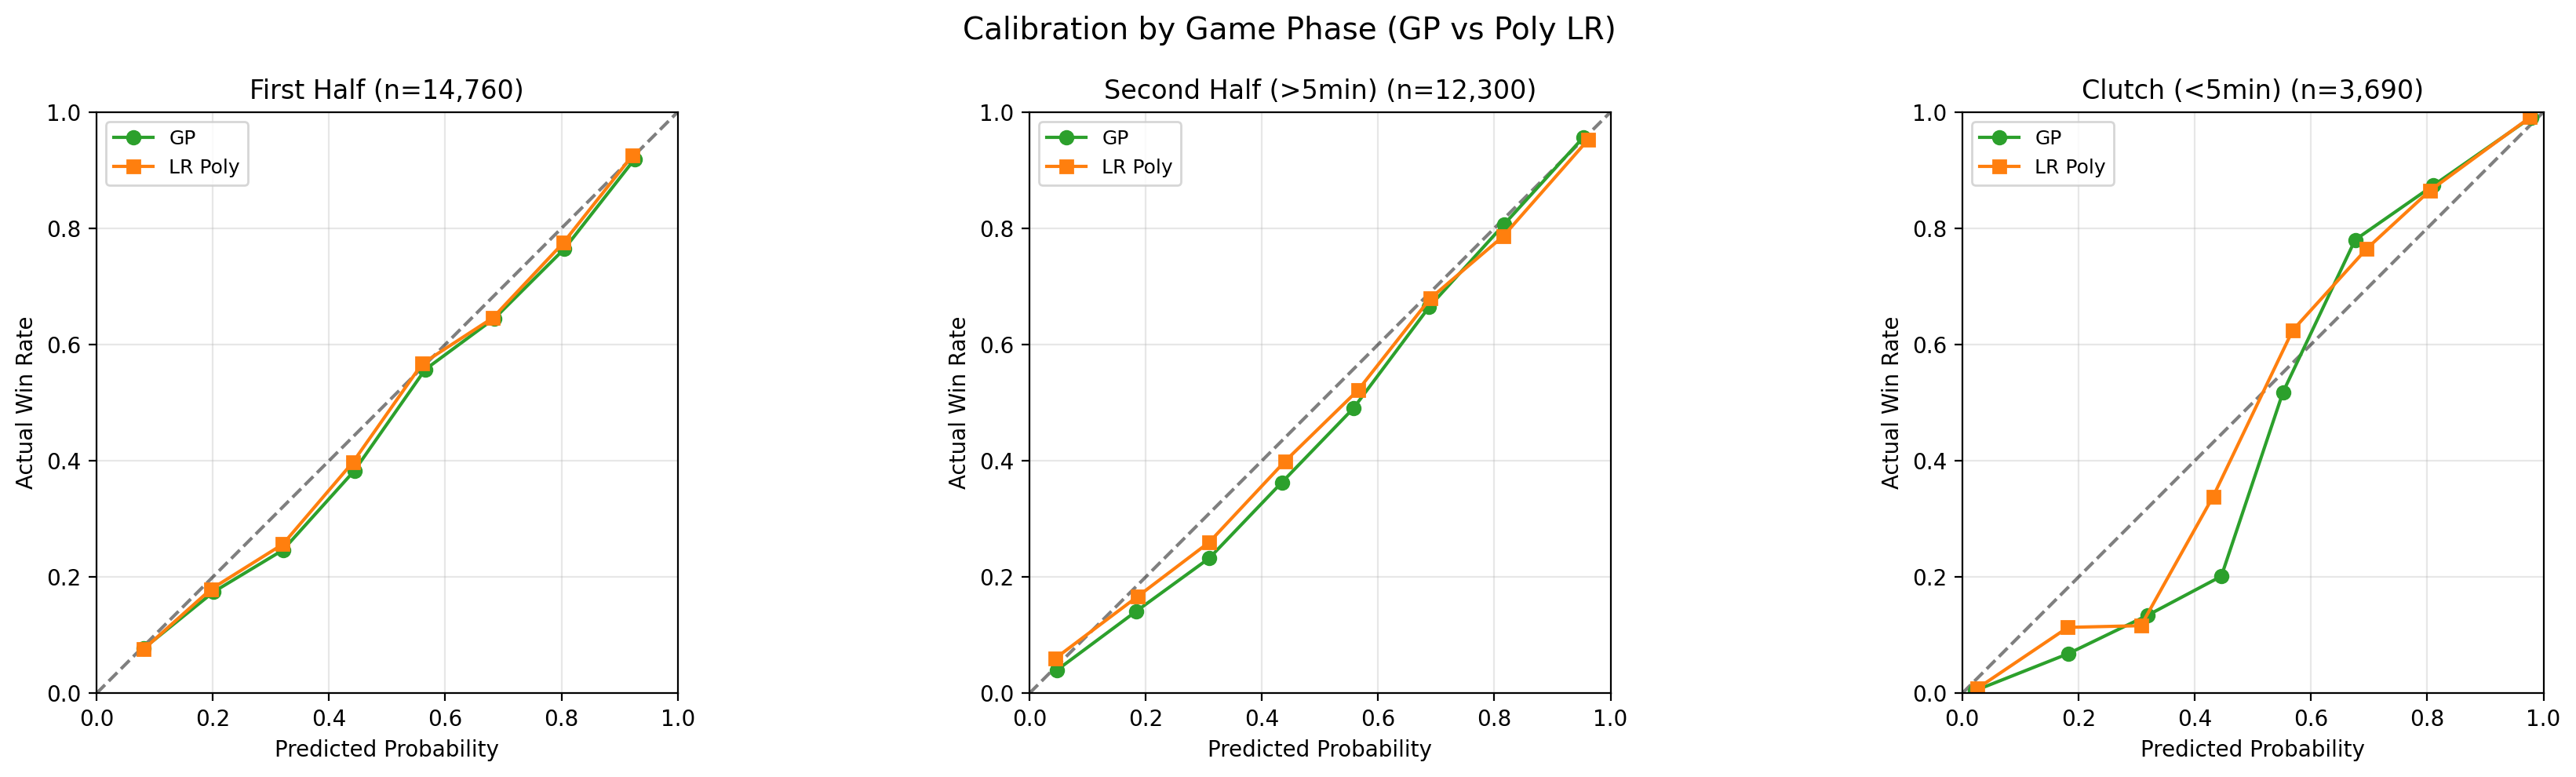
\includegraphics[width=0.92\textwidth]{figures/05_calibration_by_phase.png}
\caption{Phase-specific calibration curves comparing the GP against polynomial logistic regression across first half, second half, and clutch time.}
\label{fig:calibration_phase}
\end{figure*}

\subsection{Credible Interval Coverage}

The GP's 90\% credible intervals achieve 80\% empirical coverage, and the 95\% intervals also achieve 80\% coverage. The plateau at 80\% across both levels reflects how tightly concentrated the posterior standard deviation is: 99\% of test observations fall between 0.038 and 0.083, and the mean standard deviation within each of the 20 evaluation bins spans only 0.038 to 0.047. Widening the nominal level therefore adds little discriminative power. Sub-nominal coverage arises because the GP captures epistemic uncertainty about the win probability function but does not model the aleatoric component of binary outcome variance. The average 90\% credible interval width (posterior sharpness) is 0.1331, indicating bands spanning approximately $\pm 6.7$ percentage points around the posterior mean.

\subsection{Uncertainty Decomposition}

The decomposition of uncertainty across game contexts constitutes the study's central analytical finding. Table~\ref{tab:uncertainty} presents epistemic uncertainty (GP posterior standard deviation) alongside an aleatoric proxy defined as $0.5 - |p_{\text{pred}} - 0.5|$.

\begin{table}[t]
\centering
\caption{Epistemic vs. Aleatoric Uncertainty by Game Context}
\label{tab:uncertainty}
\begin{tabular}{lccc}
\toprule
\textbf{Context} & \textbf{Epistemic} & \textbf{Aleatoric} & \textbf{n} \\
\midrule
Blowout ($|m| \geq 15$) & 0.0480 & 0.0527 & 6{,}231 \\
Clutch ($|m| \leq 5$, $t < 5$m) & 0.0393 & 0.3142 & 988 \\
Normal & 0.0385 & 0.3145 & 23{,}531 \\
\bottomrule
\end{tabular}
\end{table}

Blowout states exhibit elevated epistemic uncertainty (sparse training data) but very low aleatoric uncertainty (the leading team almost always wins). Clutch states exhibit the inverse: low epistemic uncertainty (abundant training data near margin zero) but high aleatoric uncertainty (predicted probability near 0.5). Clutch and normal contexts show comparably high aleatoric uncertainty, 0.3142 and 0.3145 respectively, both approximately 6x higher than blowout states, so the aleatoric dimension separates decided games from undecided ones rather than clutch time from the rest of the game. This reveals information invisible to point-estimate models: a logistic regression reporting 72\% in a blowout and 53\% in a clutch scenario treats both as similarly reliable, while the GP reveals qualitatively different confidence profiles.

% === FIGURE: Epistemic vs Aleatoric ===
\begin{figure*}[!t]
\centering
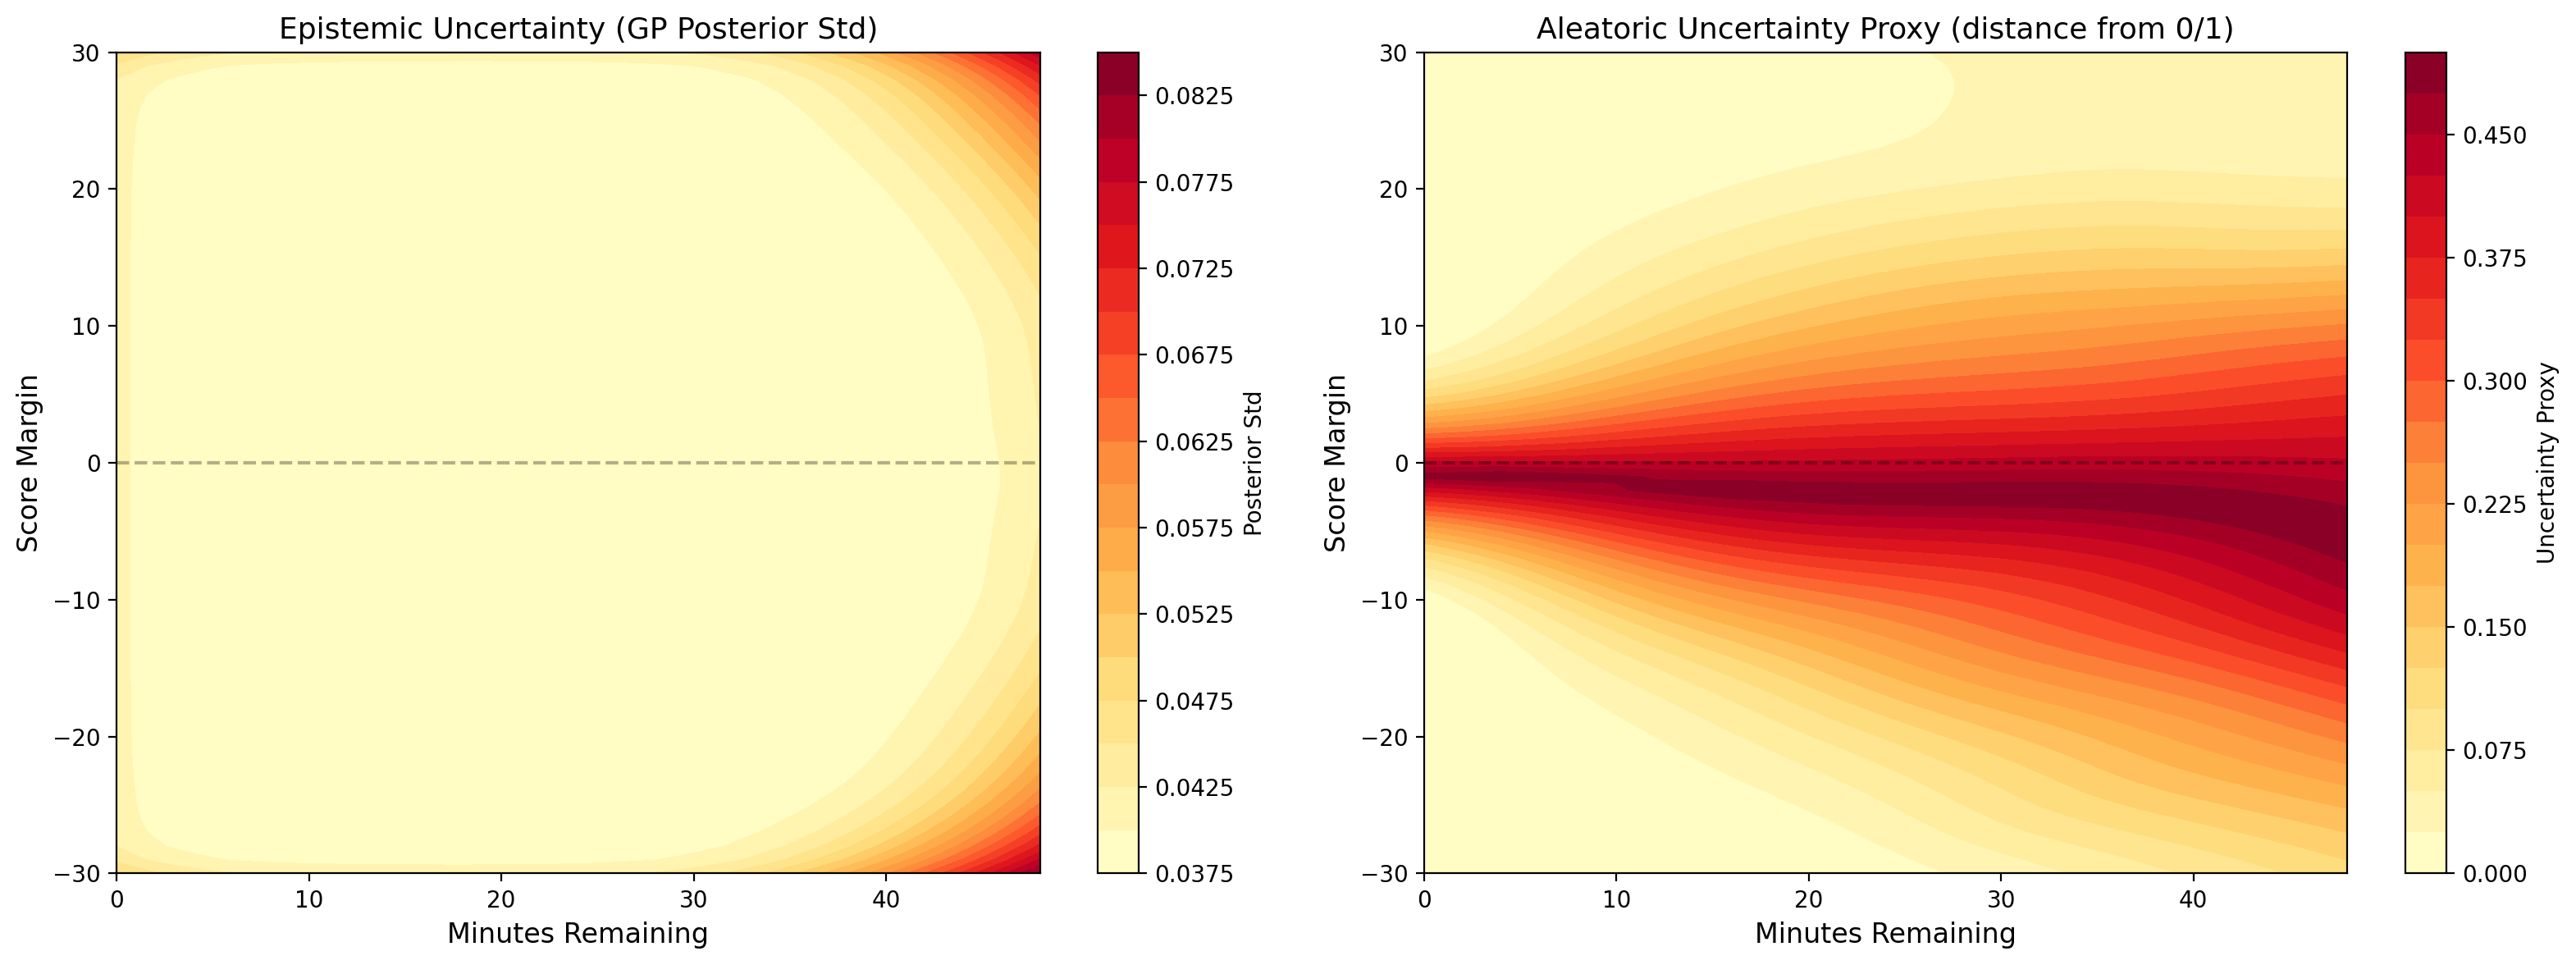
\includegraphics[width=0.92\textwidth]{figures/04_epistemic_vs_aleatoric.png}
\caption{Uncertainty decomposition surfaces. Left: epistemic uncertainty (GP posterior std), highest at extreme margins. Right: aleatoric uncertainty proxy, highest near margin zero.}
\label{fig:epistemic_aleatoric}
\end{figure*}

\subsection{Game Trajectory Overlays}

Individual game trajectories overlaid with GP credible intervals demonstrate the model's behavior across contrasting game narratives: dramatic comebacks, close finishes, and cases where the GP was confidently wrong.

% === FIGURE: Game Trajectories ===
\begin{figure*}[t]
\centering
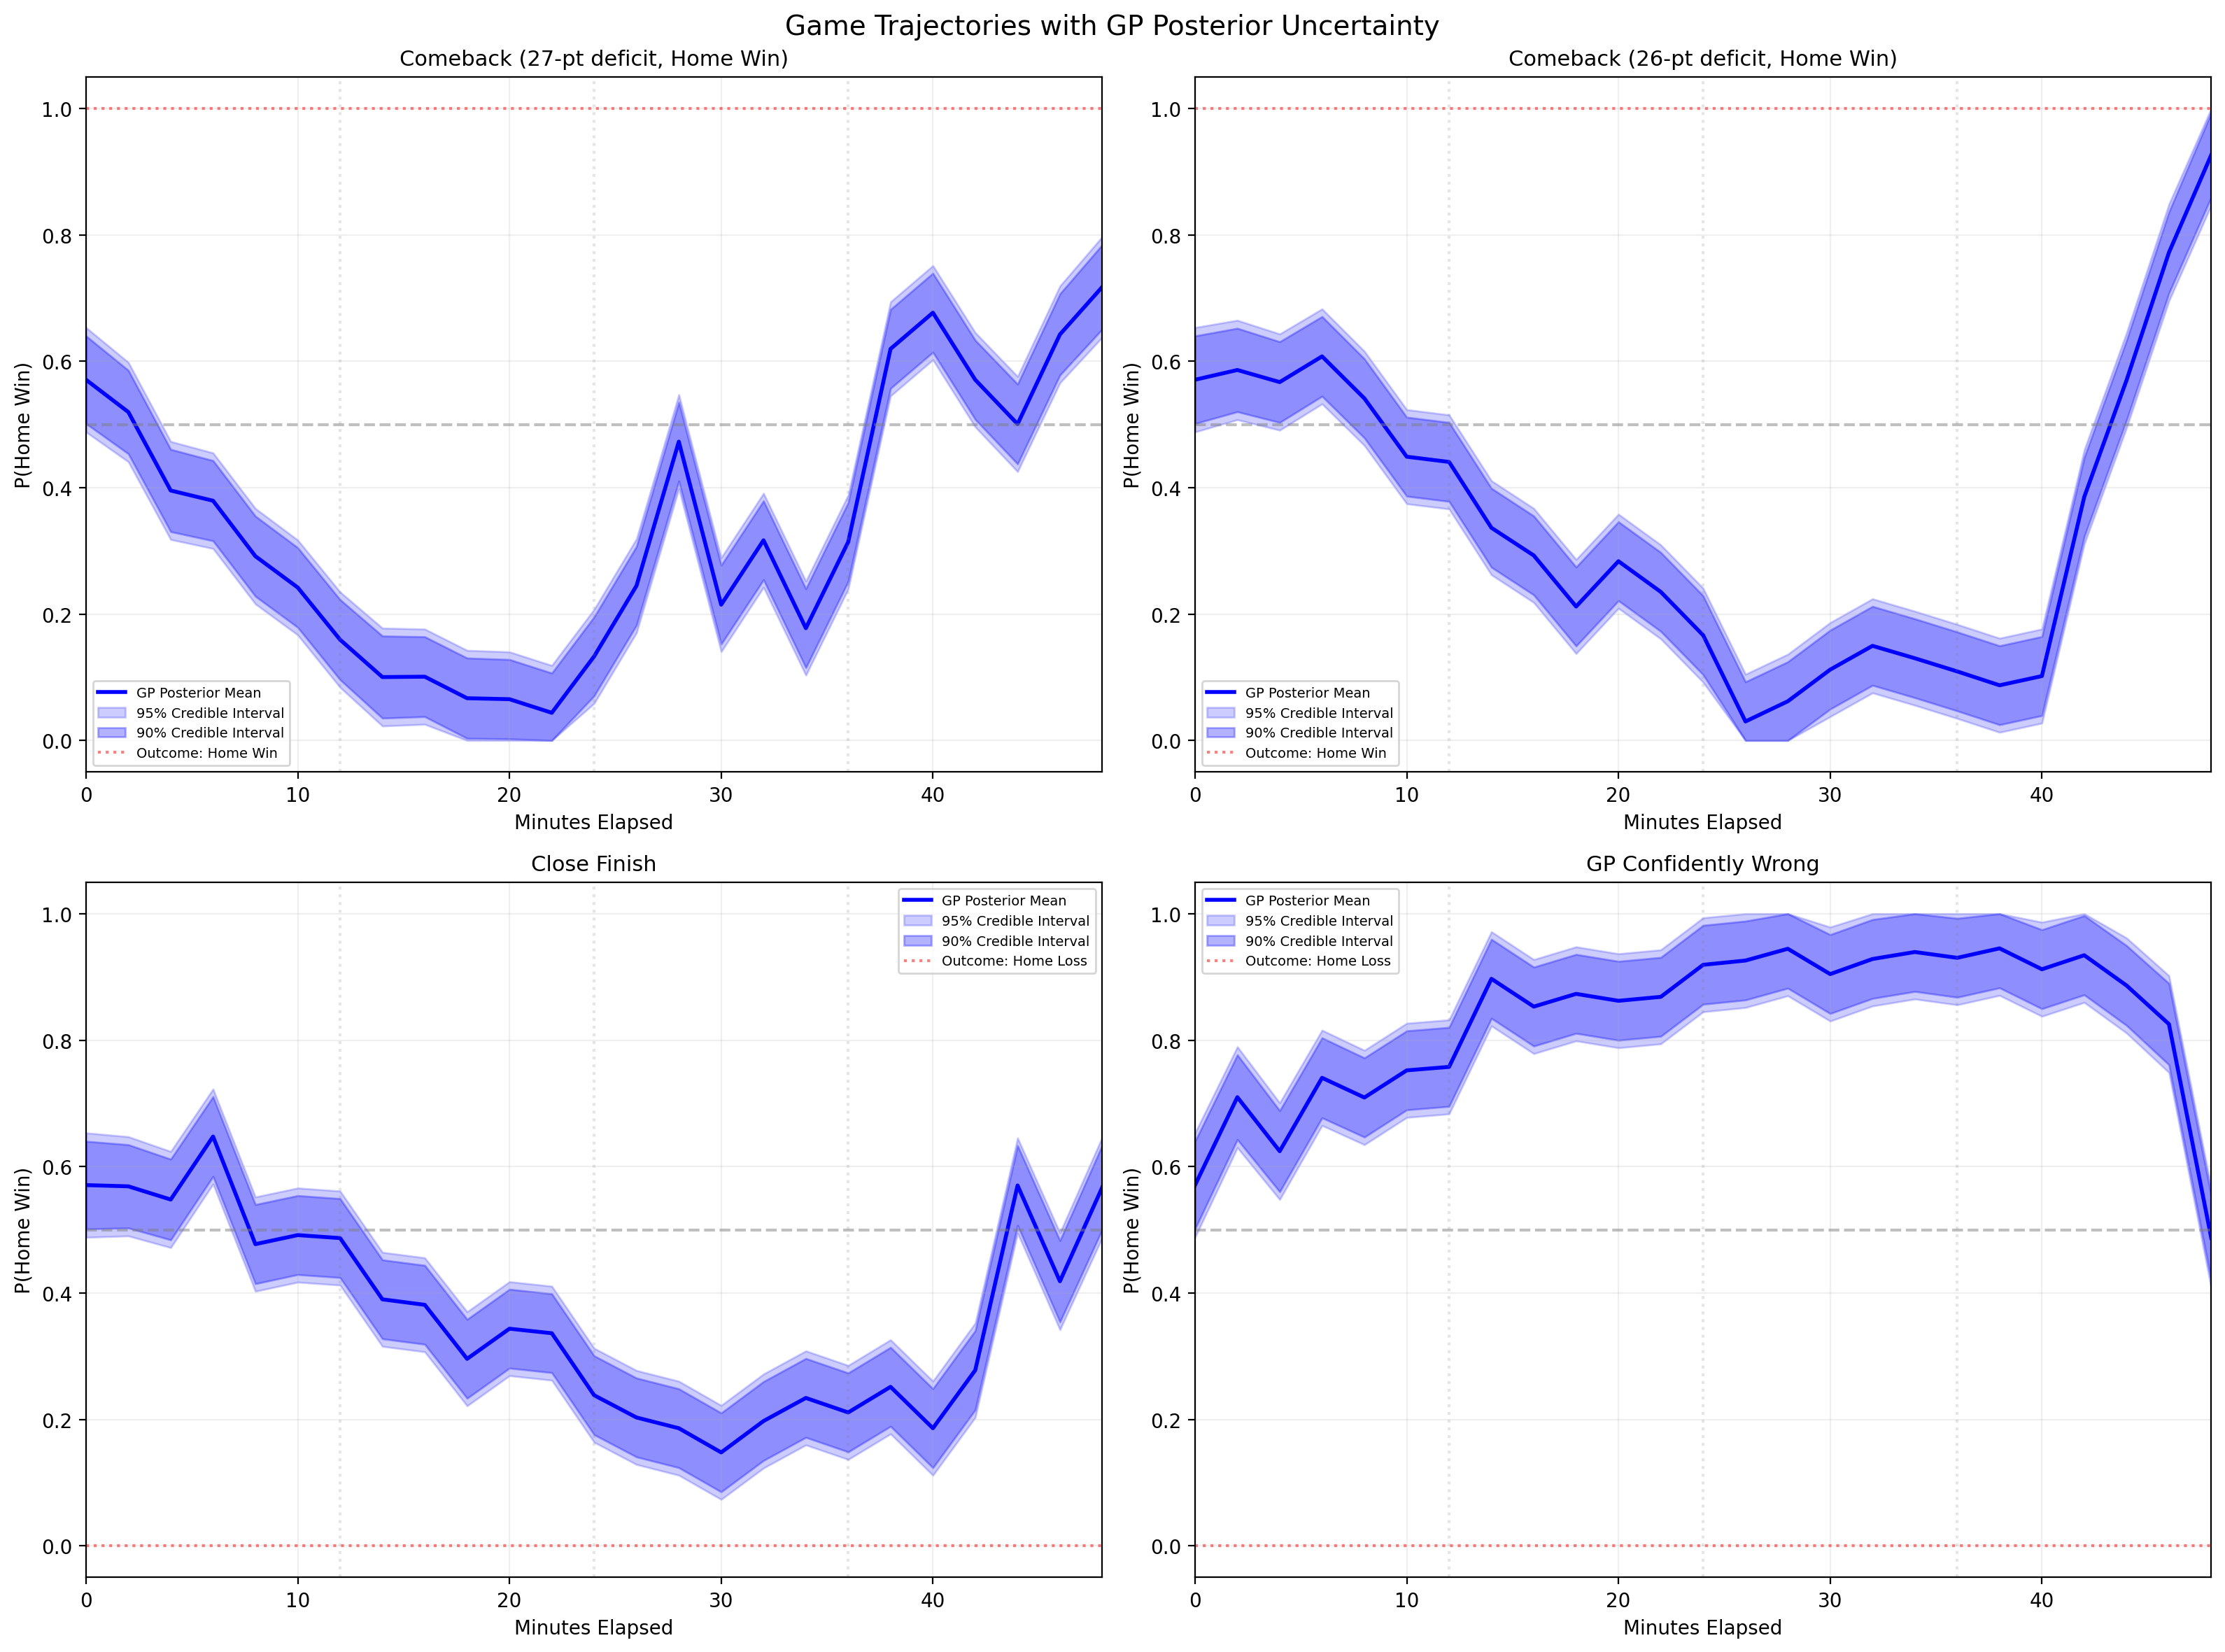
\includegraphics[width=0.92\textwidth]{figures/06_game_trajectories.png}
\caption{Game trajectories from the 2023--24 test season with GP posterior mean and 90\%/95\% credible intervals. The credible bands widen during volatile phases and narrow during stable leads, demonstrating context-sensitive uncertainty quantification.}
\label{fig:trajectories}
\end{figure*}

\subsection{Temporal Stability}

Rolling temporal validation confirms the GP's stability. When trained on 2018--22 and tested on 2022--23, the GP achieves log-loss 0.4969 (vs. 0.4973 for polynomial LR). When trained on 2018--23 and tested on 2023--24, the GP achieves 0.4819 (vs. 0.4804 for polynomial LR). Differences consistently below 0.002 indicate reliable generalization without overfitting to season-specific patterns.

\begin{table}[t]
\centering
\caption{Rolling Temporal Validation}
\label{tab:temporal}
\begin{tabular}{lcccc}
\toprule
& \multicolumn{2}{c}{\textbf{GP}} & \multicolumn{2}{c}{\textbf{LR Poly}} \\
\cmidrule(lr){2-3} \cmidrule(lr){4-5}
\textbf{Split} & Log-Loss & Brier & Log-Loss & Brier \\
\midrule
Train 18--22, Test 22--23 & 0.4969 & 0.1692 & 0.4973 & 0.1696 \\
Train 18--23, Test 23--24 & 0.4819 & 0.1633 & 0.4804 & 0.1627 \\
\bottomrule
\end{tabular}
\end{table}

% ============================================================
\section{Discussion}
% ============================================================

\subsection{Accuracy-Uncertainty Tradeoff}

The GP's primary value proposition is informational completeness, not predictive superiority. XGBoost outperforms the GP by 0.007 in log-loss, a gap small enough to be practically negligible but reproducible. The gap comes down to how each model handles transitions in the probability surface. XGBoost learns hard cutoffs, if the margin crosses a certain threshold at a certain time, the prediction jumps. The GP cannot do that because the kernel forces the surface to be smooth and continuous everywhere. In practice, this means the GP slightly underpredicts certainty in late-game scenarios where a moderate lead is effectively a guaranteed win. That said, the 0.007 difference in log-loss is a small price to pay for what you get in return: a credible interval at every game state that tells you not just the prediction, but how much the model trusts it.

\subsection{Kernel Composition as Structural Discovery}

One of the more interesting outcomes of the kernel comparison is what the optimized weights actually tell us about how basketball games unfold. The composite kernel settled at 93\% RBF and 7\% Mat\'{e}rn 1.5, which in practical terms means the GP learned that win probability evolves gradually for the vast majority of the game, possession by possession, but occasionally shifts sharply. Those sharp shifts line up with what anyone who watches basketball would recognize: a quick 8-0 run off turnovers, a dagger three in transition, or an and-one that swings a 4-point margin in one play. The GP arrived at this structure on its own through marginal likelihood optimization, without us encoding any basketball knowledge into the kernel design.

\subsection{The Epistemic-Aleatoric Distinction in Practice}

Consider two concrete game states passed through the deployed model. In a blowout with the home team leading 89--71 with 4:00 left in the third quarter, the GP predicts $P(\text{home win}) = 0.959$ with posterior standard deviation 0.0380, an aleatoric proxy of 0.0409, and a 95\% credible interval of $[0.885, 1.000]$. In a clutch situation with the home team leading 105--103 and 1:30 left in the fourth, the GP predicts $P(\text{home win}) = 0.713$ with posterior standard deviation 0.0394, an aleatoric proxy of 0.2874, and a 95\% credible interval of $[0.635, 0.790]$.

What separates these two states is almost entirely aleatoric. The epistemic terms are nearly identical, 0.0380 against 0.0394, because both states sit in densely sampled regions of the training grid: an 18-point lead in the third quarter is common, and so is a two-point lead in the final ninety seconds. The aleatoric proxy, by contrast, differs by a factor of seven. The elevated blowout epistemic uncertainty reported in Table~\ref{tab:uncertainty} is driven by the genuinely sparse corners of the surface, extreme margins early in games, not by every state that happens to be labelled a blowout.

The practical consequence is that a point-estimate model reporting 96\% and 71\% offers no mechanism to communicate why the first number is trustworthy in a different sense than the second. The GP communicates it natively through the posterior: the blowout interval is narrow and pinned against the probability ceiling, while the clutch interval is a genuine 15-point band around an outcome that is close to a coin flip on the aleatoric dimension.

% ============================================================
\section{Limitations}
% ============================================================

There are several limitations worth noting honestly, and most of them trace back to deliberate scope decisions rather than oversights.

The input space is only two-dimensional. Score margin and time remaining say nothing about which teams are playing, who is available, who is in foul trouble, or which team has the ball. A model that knows the home team is a 60-win contender and the visitor is tanking should predict differently from one that does not, and ours cannot. Adding those features is not free, though: exact GP inference costs $\mathcal{O}(n^3)$ in the number of training points, so a richer feature space would require sparse or inducing-point approximations rather than a straightforward extension of what is presented here.

The GP is fitted to binned win rates rather than to individual binary outcomes. This is an approximation of full GP classification, which would require Laplace approximation or expectation propagation to handle the non-Gaussian likelihood \cite{rasmussen2006}. Binning was chosen for computational tractability: it reduces 143,300 training observations to 634 grid points, which makes exact inference feasible on a laptop. The tradeoff is that the binning discards within-bin variation and treats each bin's empirical rate as a noisy observation of a latent smooth function, which is a modelling assumption rather than a fact about the data.

Credible interval coverage sits at 80\% for both the 90\% and 95\% nominal levels. The plateau is informative rather than mysterious. The GP's posterior variance quantifies uncertainty about the win probability function itself, and that function is well determined almost everywhere by 634 densely populated bins. What the posterior does not include is the variance of the binary outcome around that function, which is the dominant source of unpredictability in an actual game. A heteroscedastic noise model that scales with $\hat{p}(1-\hat{p})$, or a formal epistemic-aleatoric decomposition in the sense of Kendall and Gal \cite{kendall2017}, would be the natural way to close the gap.

No comparison against a proprietary model was possible. ESPN, NBA.com, and the betting markets all publish win probability curves during live games, but none archive their predictions in a form that can be downloaded and scored after the fact. Benchmarking against them would require logging predictions in real time over a full season, which was outside the timeline of this study.

Finally, the rolling temporal validation in Table~\ref{tab:temporal} was run with a Mat\'{e}rn 1.5 kernel alone rather than the composite kernel that was ultimately deployed. The two kernels differ by 2.45 in log marginal likelihood and produce very similar surfaces, so the stability conclusion is unlikely to change, but the validated architecture and the deployed architecture are not strictly identical and the results should be read with that caveat.

% ============================================================
\section{Conclusion}
% ============================================================

This study set out to test whether Bayesian Gaussian Process inference could add meaningful uncertainty information to NBA in-game win probability estimation without giving up predictive accuracy, and the answer is largely yes. On the held-out 2023--24 season the GP reaches a log-loss of 0.4831 against XGBoost's 0.4766, a gap of 0.007 that is reproducible but small enough to be irrelevant for any practical purpose, and in exchange it returns a full posterior at every game state rather than a single number.

The kernel selection procedure turned out to be more than hyperparameter tuning. Comparing five candidate priors by log marginal likelihood selected a composite RBF + Mat\'{e}rn 1.5 structure whose optimized weights, 93\% smooth and 7\% rough, describe something real about how basketball games evolve: mostly gradual drift, occasionally punctuated by scoring runs that move the margin several points at once. No basketball knowledge was encoded in the kernel design; the marginal likelihood found it.

The uncertainty decomposition is where the Bayesian treatment earns its keep. Splitting posterior uncertainty into an epistemic component, which reflects how much the model has seen of a given game state, and an aleatoric component, which reflects how genuinely undecided the outcome is, produces two numbers that behave differently across contexts and that a point estimate collapses into one. A 96\% prediction in a decided game and a 71\% prediction in a two-point game with ninety seconds left are not uncertain in the same way, and any downstream decision, whether it is a coaching choice, a broadcast graphic, or a live betting line, is better served by knowing which kind of uncertainty it is facing.

Future work should extend the feature space with team quality and availability information under a sparse GP approximation, replace the binned regression with full GP classification via approximate inference, and log predictions against a proprietary model in real time to establish an external benchmark. None of these change the central point: for the same predictive accuracy that standard tools already deliver, the GP demonstrates that the Bayesian framework surfaces information that the standard analytical toolkit leaves on the table.

% ============================================================
\begin{thebibliography}{10}

\bibitem{rasmussen2006}
C.~E. Rasmussen and C.~K.~I. Williams, \textit{Gaussian Processes for Machine Learning}. Cambridge, MA: MIT Press, 2006.

\bibitem{kendall2017}
A.~Kendall and Y.~Gal, ``What uncertainties do we need in Bayesian deep learning for computer vision?'' in \textit{Advances in Neural Information Processing Systems}, vol.~30, 2017.

\bibitem{stern1994}
H.~S. Stern, ``A Brownian motion model for the progress of sports scores,'' \textit{J. Amer. Statist. Assoc.}, vol.~89, no.~427, pp.~1128--1134, 1994.

\bibitem{lock2014}
D.~Lock and D.~Nettleton, ``Using random forests to estimate win probability before each play of an NFL game,'' \textit{J. Quant. Anal. Sports}, vol.~10, no.~2, pp.~197--205, 2014.

\bibitem{cervone2016}
D.~Cervone, A.~D'Amour, L.~Bornn, and K.~Goldsberry, ``A multiresolution stochastic process model for predicting basketball possession outcomes,'' \textit{J. Amer. Statist. Assoc.}, vol.~111, no.~514, pp.~585--599, 2016.

\bibitem{thabtah2019}
F.~Thabtah, L.~Zhang, and N.~Abdelhamid, ``NBA game result prediction using feature analysis and machine learning,'' \textit{Annals of Data Science}, vol.~6, no.~1, pp.~103--116, 2019.

\bibitem{frazier2018}
P.~I. Frazier, ``A tutorial on Bayesian optimization,'' \textit{arXiv preprint arXiv:1807.02811}, 2018.

\bibitem{bishop2006}
C.~M. Bishop, \textit{Pattern Recognition and Machine Learning}. New York: Springer, 2006.

\bibitem{chen2016}
T.~Chen and C.~Guestrin, ``XGBoost: A scalable tree boosting system,'' in \textit{Proc. 22nd ACM SIGKDD Int. Conf. Knowl. Discov. Data Mining}, 2016, pp.~785--794.

\bibitem{pedregosa2011}
F.~Pedregosa \textit{et al.}, ``Scikit-learn: Machine learning in Python,'' \textit{J. Mach. Learn. Res.}, vol.~12, pp.~2825--2830, 2011.

\bibitem{pilario2023}
K.~E. Pilario, ``AI 221: Machine Learning, Lecture Notes Weeks 2--10,'' University of the Philippines Diliman, 2023.

\end{thebibliography}

\end{document}
